\section{Fixed-point theory} 
A fixed-point of a function is an element in the domain of that function such that the function maps to itself for that element. Fixed-points are used in model verification as well as in some parity game algorithms.

Fixed-point theory goes hand in hand with lattice theory which we introduce first.
\subsection{Lattices}
We introduce definitions for ordering and lattices taken from \cite{birkhoff1940lattice}.
\begin{definition}[\cite{birkhoff1940lattice}]
	A partial order is a binary relation $x \leq y$ on set $S$ where for all $x,y,z \in S$ we have:
	\begin{itemize}
		\item $x \leq x$. (Reflexive)
		\item If $x \leq y$ and $y \leq x$, then $x=y$. (Antisymmetric)
		\item If $x \leq y$ and $y \leq z$, then $x \leq z$. (Transitive)
	\end{itemize}
\end{definition}

\begin{definition}[\cite{birkhoff1940lattice}]
	A partially ordered set is a set $S$ and a partial order $\leq$ for that set, we denote a partially ordered set by $\langle S, \leq \rangle$.
\end{definition}

\begin{definition}[\cite{birkhoff1940lattice}]
	Given partially ordered set $\langle P,\leq \rangle$ and subset $X \subseteq P$. An upper bound to $X$ is an element $a \in P$ such that $x \leq a$ for every $x\in X$. A least upper bound to $X$ is an upper bound $a \in P$ such every other upper bound is larger or equal to $a$.
\end{definition}
The term least upper bound is synonymous with the term supremum, we write $\sup \{ S \}$ to denote the supremum of set $S$.
\begin{definition}[\cite{birkhoff1940lattice}]
	Given partially ordered set $\langle P,\leq \rangle$ and subset $X \subseteq P$. A lower bound to $X$ is an element $a \in P$ such that $a \leq x$ for every $x\in X$. A greatest lower bound to $X$ is a lower bound $a \in P$ such that every other lower bound is smaller or equal to $a$.
\end{definition}
The term greatest lower bound is synonymous with the term infimum, we write $\inf \{ S\}$ to denote the infimum of set $S$.

\begin{definition}[\cite{birkhoff1940lattice}]
	A lattice is a partially ordered set where any two of its elements have a supremum and an infimum.
\end{definition}

\begin{definition}[\cite{birkhoff1940lattice}]
	A complete lattice is a partially ordered set in which every subset has a supremum and an infimum.
\end{definition}

\begin{definition}[\cite{birkhoff1940lattice}]
	Given a lattice $\langle D, \leq \rangle$, function $f : D \rightarrow D$ is monotonic if for all $x \in D$ and $y \in D$ it holds that if $x \leq y$ then $f(x) \leq f(y)$.
\end{definition}
\subsection{Fixed-points}
Fixed-points are formally defined as follows:
\begin{definition}
	Given function $f : D \rightarrow D$ the value $x \in D$ is a fixed-point for $f$ if and only if $f(x) = x$. Furthermore $x$ is the least fixed-point for $f$ if every other fixed-point for $f$ is greater or equal to $x$ and dually $x$ is the greatest fixed-point for $f$ if every other fixed-point $f$ is less or equal to $x$.
\end{definition}
The Knaster-Tarski theorem states that least and greatest fixed-points exist for some domain and function given that a few conditions hold.
The theorem, as written down by Tarski in \cite{tarski1955}, states:
\begin{theorem}[Knaster-Tarski\cite{tarski1955}]
	\label{the_knaster_tarski}
	Let
	\begin{itemize}
		\item $\langle A, \leq \rangle$ be a complete lattice,
		\item $f$ be a monotonic function on $A$ to $A$,
		\item $P$ be the set of all fixpoints of f.
	\end{itemize}
	Then the set $P$ is not empty and the system $\langle P, \leq \rangle$ is a complete lattice; in particular we have 
	\[ \sup P = \sup \{ x\ |\ f(x) \geq x \} \in P \]
	and
	\[ \inf P = \inf \{ x\ |\ f(x) \leq x \} \in P \]
\end{theorem}

\section{Model verification}
It is difficult to develop correct software, one way to improve reliability of software is through model verification; the behaviour of software is specified in a model and formal verification techniques are used to show that the behaviour adheres to certain requirements. In this section we inspect how to model behaviour and how to specify requirements.

Behaviour can be modelled as a \textit{labelled transition system} (LTS). An LTS consists of states in which the system can find itself and transitions between states. Transitions represent the possible state change of the system. Transitions are labelled with actions that indicate what kind of change is happening. Formally we define an LTS as follows.
\begin{definition}[\cite{Groote}]
	\label{def_lts}
	A labelled transition system (LTS) is a tuple $M = (S, Act, trans, s_0)$, where:
	\begin{itemize}
		\item $S$ is a finite set of states,
		\item $Act$ a finite set of actions,
		\item $trans \subseteq S \times Act \times S$ is the transition relation with $(s,a,s') \in trans$ denoted by $s \xrightarrow a s'$,
		\item $s_0 \in S$ is the initial state.
	\end{itemize}
\end{definition}

An LTS is usually depicted as a graph where the vertices represent the states, the edges represent the transitions, edges are labelled with actions and an edge with no origin vertex indicates the initial state. Such a representation is depicted in the example below.
\begin{example}[\cite{FamBasedModelCheckingWithMCRL2}]
	Consider the behaviour of a coffee machine that accepts a coin after which it serves a standard coffee, this can be repeated infinitely often. 
	
	The behaviour can be modelled as an LTS that has two states: in the initial state it is ready to accept a coin and in the second state it is ready to serve a standard coffee. We introduce two actions: \textit{ins}, which represents a coin being inserted, and \textit{std}, which represents a standard coffee being served. We get the following LTS which is also depicted in Figure \ref{fig:coffeemachinebasiceurolts}.
	\[ (\{s_1,s_2\},\{std,ins\},\{(s_1,ins,s_2),(s_2,std,s_1)\},s_1)\]
	\begin{figure}[h]
		\centering
		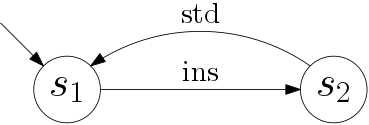
\includegraphics[scale=0.3]{Examples/CoffeeMachine/BasicEuroLTS}
		\caption[Coffee machine LTS]{Coffee machine LTS $C$}
		\label{fig:coffeemachinebasiceurolts}
	\end{figure}
\end{example}

LTSs might be non-deterministic, meaning that from a state there might be multiple transitions that can be taken, moreover multiple transitions with the same action can be taken. This is depicted in the example below.

\begin{example}
	We extend the coffee machine example where at some point the coffee machine can be empty and needs a fill before the system is ready to receive a coin again. This LTS is depicted in Figure \ref{fig:coffeemachineundeterministic}. When the \textit{std} transition is taken from state $s_2$ it is non-determined in which states the system ends.
	\begin{figure}[h]
		\centering
		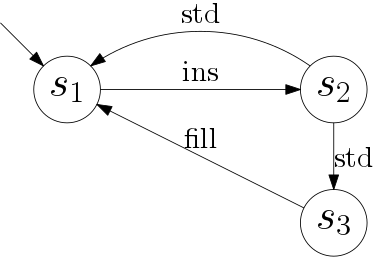
\includegraphics[scale=0.3]{Examples/CoffeeMachine/NonDeterministicEuroLTS}
		\caption[Coffee machine LTS]{Coffee machine with non-deterministic behaviour}
		\label{fig:coffeemachineundeterministic}
	\end{figure}
\end{example}


A system can be verified by checking if its behaviour adheres to certain requirements. The behaviour can be modelled in an LTS. Requirements can be expressed in a temporal logic; with a temporal logic we can express certain propositions with a time constraint such as \textit{always}, \textit{never} or \textit{eventually}. For example (relating to the coffee machine example) we can express the following constraint: "After a coin is inserted the machine always serves a standard coffee immediately afterwards". The most expressive temporal logic is the modal $\mu$-calculus. A modal $\mu$-calculus formula is expressed over a set of actions and a set of variables.

We define the syntax of the modal $\mu$-calculus below. Note that the syntax is in positive normal form, ie. no negations.
\begin{definition}[\cite{Groote}]
	\label{def_mu_syntax}
	A modal $\mu$-calculus formula over the set of actions $Act$ and a set of variables $\mathcal{X}$ is defined by
	\[ \varphi = \top\ |\ \bot\ |\ X\ |\ \varphi \vee \varphi\ |\ \varphi \wedge \varphi\ |\ \langle a \rangle \varphi\ |\ [a]\varphi\ |\ \mu X.\varphi\ |\ \nu X.\varphi \]
	with $a \in Act$ and $X \in \mathcal{X}$. 
\end{definition}
The modal $\mu$-calculus contains boolean constants $\top$ and $\bot$, propositional operators $\vee$ and $\wedge$, modal operators $\langle \, \rangle$ and $[ \, ]$ and fixpoint operators $\mu$ and $\nu$. 

A variable $X \in \mathcal{X}$ \textit{occurs free} in formula $\phi$ if and only if $X$ occurs in $\phi$ such that $X$ is not a sub-formula of $\mu X.\phi'$ or $\nu X.\phi'$ in $\phi$. A formula is \textit{closed} if and only if there are no variables that occurs free.

A formula can be interpreted in the context of an LTS, such an interpretation results in a set of states in which the formula holds. Given formula $\varphi$ we define the interpretation of $\varphi$ as $\llbracket \varphi \rrbracket ^\eta  \subseteq S$ where $\eta : \mathcal{X}\rightarrow 2^S$ maps a variable to a set of states. We can assign $S' \subseteq S$ to variable $X$ in $\eta$ by writing $\eta[X:=S']$, ie. $(\eta[X:=S'])(X) = S'$.
\begin{definition}
	\label{def_mu_sem} For LTS $(S, Act, trans, s_0)$ we inductively define the interpretation of a modal $\mu$-calculus formula $\varphi$, notation
	$\llbracket \varphi \rrbracket^\eta$, where $\eta : \mathcal{X} \rightarrow \mathcal{P}(S)$ is a variable valuation, as a set of states
	where $\varphi$ is valid, by:
	\begin{align*}
	&\llbracket {\top} \rrbracket^\eta &&= S\\
	&\llbracket {\bot} \rrbracket^\eta &&= \emptyset\\
	&\llbracket \varphi_1 \wedge \varphi_2 \rrbracket^\eta &&= \llbracket \varphi_1 \rrbracket^\eta \cap \llbracket \varphi_2 \rrbracket^\eta \\
	&\llbracket \varphi_1 \vee \varphi_2 \rrbracket^\eta &&= \llbracket \varphi_1 \rrbracket^\eta \cup \llbracket \varphi_2 \rrbracket^\eta\\
	&\llbracket \langle a \rangle \varphi \rrbracket^\eta &&= \{s \in S|\exists_{s' \in S}\ s \xrightarrow {a} s' \wedge s' \in \llbracket \varphi \rrbracket^\eta\}\\
	&\llbracket [ a ] \varphi \rrbracket^\eta &&= \{s \in S|\forall_{s' \in S}\ s \xrightarrow {a} s' \implies s' \in \llbracket \varphi \rrbracket^\eta\}\\
	&\llbracket \mu X. \varphi \rrbracket^\eta &&= \bigcap\{f \subseteq S | f \supseteq \llbracket \varphi \rrbracket^{\eta[X:=f]}\}\\
	&\llbracket \nu X. \varphi \rrbracket^\eta &&= \bigcup\{f \subseteq S | f \subseteq \llbracket \varphi \rrbracket^{\eta[X:=f]}\}\\
	&\llbracket X \rrbracket^\eta &&= \eta(X)
	\end{align*}
\end{definition}
Since there are no negations in the syntax we find that every modal $\mu$-calculus formula is monotone, ie. if we have for $U \subseteq S$ and $U' \subseteq S$ that $U \subseteq U'$ holds then $\llbracket \varphi \rrbracket^{\eta[X:=U]} \subseteq \llbracket \varphi \rrbracket^{\eta[X:=U']}$ holds for any variable $X \in \mathcal{X}$. Using the Knaster-Tarski theorem (Theorem \ref{the_knaster_tarski}) we find that the least and greatest fixed-points always exist.

Given closed formula $\varphi$, LTS $M = (S, Act, trans, s_0)$ and $s \in S$ we say that $M$ satisfies formula $\varphi$ in state $s$, and write $(M,s) \models \varphi$, if and only if $s \in \llbracket \varphi \rrbracket^\eta$. If and only if $M$ satisfies $\varphi$ in the initial state do we say that $M$ satisfies formula $\varphi$ and write $M \models \varphi$. 

\begin{example}[\cite{FamBasedModelCheckingWithMCRL2}]
	Consider the coffee machine example from Figure \ref{fig:coffeemachinebasiceurolts} and formula $\varphi = \nu X. \mu Y([inst]Y \wedge [std]X)$ which states that action \textit{std} must occur infinitely often over all infinite runs. Obviously this holds for the coffee machine, therefore we have $C \models \varphi$.
\end{example}

\section{Parity games}
A \textit{parity game} is a game played by two players: player 0 (also called player \textit{even}) and player 1 (also called player \textit{odd}). We write $\alpha \in \{0,1\}$ to denote an arbitrary player and $\overline{\alpha}$ to denote $\alpha$'s opponent, ie. $\overline{0} = 1$ and $\overline{1} = 0$. A parity game is played on a playing field which is a directed graph where every vertex is owned by either player 0 or player 1. Furthermore every vertex has a natural number, called its \textit{priority}, associated with it.
\begin{definition}[\cite{Bradfield2018}]
	\label{def_PG}
	A parity game is a tuple $(V, V_0, V_1, E, \Omega)$, where:
	\begin{itemize}
		\item $V$ is a finite set of vertices partitioned in sets $V_0$ and $V_1$, containing vertices owned by player 0 and player 1 respectively,
		\item $E \subseteq V \times V$ is the edge relation,
		\item $\Omega :  V \rightarrow \mathbb{N}$ is the priority assignment function.
	\end{itemize}
\end{definition}
Parity games are usually represented as a graph where vertices owned by player 0 are shown as diamonds and vertices owned by player 1 are shown as boxes, furthermore the priorities are depicted as numbers inside the vertices. Such a representation is shown in the example below.

\begin{example}
	Figure \ref{fig:simplepgpg} shows the parity game:
	\[ V_0 = \{v_1,v_4,v_5\},V_1 = \{v_2,v_3\}, V = V_0 \cup V_1\]
	\[ E = \{(v_1,v_2),(v_2,v_1),(v_1,v_3),(v_2,v_4),(v_3,v_4),(v_3,v_5),(v_4,v_4)\}\] 
	\[ \Omega = \{v_1 \mapsto 2, v_2 \mapsto 3, v_3 \mapsto 0, v_4 \mapsto 0, v_5 \mapsto 1 \}\]
	\begin{figure}[h]
		\centering
		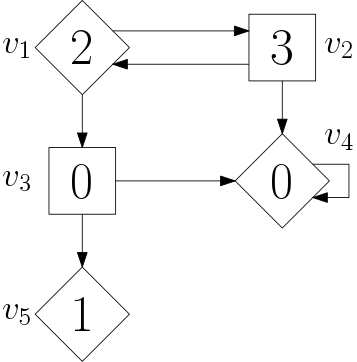
\includegraphics[scale=0.3]{Examples/SimplePG/PG}
		\caption[Parity game example]{Parity game example}
		\label{fig:simplepgpg}
	\end{figure}
\end{example}

A parity game can be played for a vertex $v \in V$. We start by placing a token on vertex $v$, the player that owns vertex $v$ can choose to move the token along an edge to a vertex $w \in V$ such that $(v,w) \in E$. Again the player that owns vertex $w$ can choose where to move the token next. This is repeated either infinitely often or until a player cannot make a move, ie. the token is on a vertex with no outgoing edges. Playing in this manner gives a sequence of vertices, called a \textit{path}, starting from vertex $v$. For path $\pi$ we write $\pi_i$ to denote $i^\text{th}$ vertex in path $\pi$. Every path is associated with a winner (either player 0 or 1). If a player $\alpha$ cannot move at some point we get a finite path and player $\overline{\alpha}$ wins the path. If we get an infinite path $\pi$ then the winner is determined by the parity of the highest priority that occurs infinitely often in the path. Formally we determine the highest priority occurring infinitely often by the following formula.
\[ \max\{ p \ |\ \forall_j \exists_i j < i \wedge p = \Omega(\pi_i) \}\] 
If the highest priority is odd then player $1$ wins the path, if it is even player $0$ wins the path.

A path is \textit{valid} if and only if for every $i > 0$ such that $\pi_i$ exists we have $(\pi_{i-1},\pi_i) \in E$.


\begin{example}
	Again consider the example in Figure \ref{fig:simplepgpg}. If we play the game for vertex $v_1$ we start by placing a token on $v_1$. Consider the following exemplary paths where $(w_1{\dots}w_m)^\omega$ indicates an infinite repetition of vertices $w_1{\dots}w_m$.
	\begin{itemize}
		\item $\pi = v_1v_3v_5$ is won by player $1$ since player $0$ cannot move at $v_5$.
		\item $\pi = (v_1v_2)^\omega$ is won by player $1$ since the highest priority occurring infinitely often is 3.
		\item $\pi = v_1v_3(v_4)^\omega$ is won by player $0$ since the highest priority occurring infinitely often is $0$.
	\end{itemize}
\end{example}

The moves that the players make are determined by their \textit{strategies}. A strategy $\sigma_\alpha$ determines for a vertex in $V_\alpha$ where the token goes next. We can define a strategy for player $\alpha$ as a partial function $\sigma_\alpha : V^*V_\alpha \rightarrow V$ that maps a series of vertices ending with a vertex owned by player $\alpha$ to the next vertex such that for any $\sigma_\alpha(w_0\dots w_m) = w$ we have $(w_m,w) \in E$. A path $\pi$ \textit{conforms to} strategy $\sigma_\alpha$ if for every $i > 0$ such that $\pi_i$ exists and $\pi_{i-1} \in V_\alpha$ we have $\pi_i = \sigma_\alpha(\pi_0\pi_1\dots\pi_{i-1})$.

A strategy is \textit{winning} for player $\alpha$ from vertex $v$ if and only if $\alpha$ is the winner of every valid path starting in $v$ that conforms to $\sigma_\alpha$. If such a strategy exists for player $\alpha$ from vertex $v$ we say that vertex $v$ is winning for player $\alpha$.

\begin{example}
	In the parity game seen in Figure \ref{fig:simplepgpg} vertex $v_1$ is winning for player 1. Player 1 has a strategy that plays every vertex sequence ending in $v_2$ to $v_1$ and plays every vertex sequence ending in $v_3$ to $v_5$. Regardless of the strategy for player 0 the path will either end up in $v_5$ or will pass $v_2$ infinitely often. In the former case player 1 wins the path because player 0 can not move at $v_5$. In the latter case the highest priority occurring infinitely often is 3.
\end{example}

Parity games are known to be positionally determined \cite{Bradfield2018}, meaning that every vertex in a parity game is winning for one of the two players. Also every player has a \textit{positional strategy} that is winning starting from each of his/her winning vertices. A positional strategy is a strategy that only takes the current vertex into account to determine the next vertex, it does not look at already visited vertices. Therefore we can consider a strategy for player $\alpha$ as a complete functions $\sigma_\alpha : V_\alpha \rightarrow V$. Finally it is decidable for each of the vertices in a parity who the winner is \cite{Bradfield2018}.

A parity game is \textit{solved} if the vertices are partitioned in two sets, namely $W_0$ and $W_1$, such that every vertex in $W_0$ is winning for player 0 and every vertex in $W_1$ is winning for player 1. We call these sets the \textit{winning sets} of a parity game.

Finally parity games are considered \textit{total} if and only if every vertex has at least one outgoing edge. Playing a total parity game always results in an infinite path. We can make a non-total parity game total by adding two sink vertices: $l_0$ and $l_1$. Each sink vertex has only one outgoing edge, namely to itself. Vertex $l_0$ has priority 1 and vertex $l_1$ has priority 0. Clearly if the token ends up in $l_\alpha$ then player $\alpha$ looses the game because with only one outgoing edge we only get a single priority that occurs infinitely often, namely priority $\overline{\alpha}$. For every vertex $v \in V_\alpha$ that does not have an outgoing edge we create an edge from $v$ to $l_\alpha$. In the original game player $\alpha$ lost when the token was in vertex $v$ because he/she could not move any more. In the total game player $\alpha$ can only play to $l_\alpha$ from $v$ where he/she still looses. So using this method vertices in the total game have the same winner as they had in the original game (except for $l_0$ and $l_1$ which did not exist in the original game). In general we try to only work with total games because no distinction is required between finite paths and infinite paths when reasoning about them, however we will encounter some scenario's where non-total games are still considered.

\subsection{Relation between parity games and model checking}
Verifying LTSs against a modal $\mu$-calculus formula can be done by solving a parity game. This is done by translating an LTS in combination with a formula to a parity game, the solution of the parity game provides the information needed to conclude if the model satisfies the formula. This relation is depicted in figure \ref{fig:ltsverificationusingpg}. 
\begin{figure}[h]
	\centering
	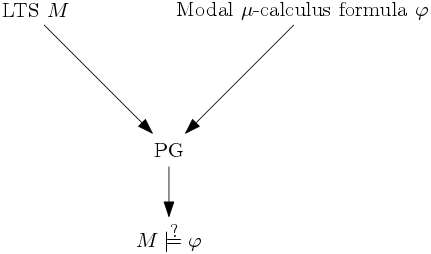
\includegraphics[scale=0.5]{Diagrams/LTSVerificationUsingPG}
	\caption[LTS verification using PG]{LTS verification using PG}
	\label{fig:ltsverificationusingpg}
\end{figure}

We consider a method of creating parity games from an LTS and a modal $\mu$-calculus formula such that there is a special vertex $w$ in the parity game that indicates if the LTS satisfies the formula; if and only if $w$ is won by player 0 is the formula satisfied.

First we introduce the notion of unfolding. A fixpoint formula $\mu X . \varphi$ can be unfolded, resulting in formula $\varphi$ where every occurrence of $X$ is replaced by $\mu X . \varphi$, denoted by $\varphi [ X:= \mu X . \varphi]$. Interpreting a fixpoint formula results in the same set as interpreting its unfolding as shown in \cite{Bradfield2018}; i.e. $[\![\mu X . \varphi]\!]^\eta = [\![\varphi[X:=\mu X . \varphi]]\!]^\eta$. The same holds for the fixpoint operator $\nu$.

Next we define the Fischer-Ladner closure for a closed $\mu$-calculus formula 
\cite{STREETT1989249,FISCHER1979194}. The Fischer-Ladner closure of $\varphi$ is the set $\textit{FL}(\varphi)$ of closed formulas containing at least $\varphi$. Furthermore for every formula $\psi$ in $\textit{FL}(\varphi)$ it holds that for every direct subformula $\psi'$ of $\psi$ there is a formula in $\textit{FL}(\varphi)$ that is equivalent to $\psi'$.
\begin{definition}
	\label{def_FLClosure}
	The Fischer-Ladner closure of closed $\mu$-calculus formula $\varphi$ is the smallest set $\textit{FL}(\varphi)$ satisfying the following constraints:
	\begin{itemize}
		\item $\varphi \in \textit{FL}(\varphi)$,
		\item if $\varphi_1 \vee \varphi_2 \in \textit{FL}(\varphi)$ then $\varphi_1 ,\varphi_2 \in \textit{FL}(\varphi)$,
		\item if $\varphi_1 \wedge \varphi_2 \in \textit{FL}(\varphi)$ then $\varphi_1 ,\varphi_2 \in \textit{FL}(\varphi)$,
		\item if $\langle a \rangle \varphi' \in \textit{FL}(\varphi)$ then $\varphi' \in \textit{FL}(\varphi)$,
		\item if $[ a ] \varphi' \in \textit{FL}(\varphi)$ then $\varphi' \in \textit{FL}(\varphi)$,
		\item if $\mu X . \varphi' \in \textit{FL}(\varphi)$ then $\varphi'[X:= \mu X . \varphi'] \in \textit{FL}(\varphi)$ and
		\item if $\nu X . \varphi' \in \textit{FL}(\varphi)$ then $\varphi'[X:= \nu X . \varphi'] \in \textit{FL}(\varphi)$.
		
	\end{itemize}
\end{definition}

We also define the alternation depth of a formula.
\begin{definition}[\cite{Bradfield2018}]
	The dependency order on bound variables of $\varphi$	is the smallest partial order such that $X \leq_\varphi Y$ if $X$ occurs free in $\sigma Y. \psi$ . The alternation depth of a $\mu$-variable X in formula $\varphi $ is the maximal length of a chain $X_1 \leq_\varphi  \dots \leq_\varphi X_n$ where $X = X_1$, variables $X_1, X_3, \dots$ are $\mu$-variables and variables $X_2, X_4, \dots$ are $\nu$-variables. The alternation depth of a $\nu$-variable is defined similarly. The alternation depth of formula $\varphi$, denoted $adepth(\varphi)$, is the maximum of the alternation depths of the variables bound in $\varphi$, or zero if there are no fixpoints.
\end{definition}
\begin{example}
	Consider the formula $\varphi = \nu X. \mu Y. ([ins]Y \wedge [std] X)$ which states that for an LTS with $Act = \{ ins, std\}$ the action \textit{std} must occur infinitely often over all infinite runs. Since $X$ occurs free in $\mu Y. ([ins] Y \wedge [std]X)$ we have $adepth(Y) = 1$ and $adepth(X) = 2$.
\end{example}
As shown in \cite{Bradfield2018} it holds that formula $\mu X. \psi$ has the same alternation depth as its unfolding $\psi[X:=\mu X. \psi]$. Similarly for the greatest fixpoint. 

Next we define the transformation from an LTS and a formula to a parity game.
\begin{definition}[\cite{Bradfield2018}]
	\label{def_LTS2PG}
	LTS2PG($M, \varphi$) converts LTS $M = (S, Act, trans, s_0)$ and closed formula $\varphi$ to a parity game $(V, V_0, V_1, E, \Omega)$.
	
	Vertices in the parity game are presented as pairs of states and sub-formulas. A vertex is created for every state with every formula in the Fischer-Ladner closure of $\varphi$. We define the set of vertices:
	\[ V = S \times \textit{FL}(\varphi) \]
	
	Vertices have the following owner and successors:\\
	\begin{center}
		\begin{tabular}{l|l|l}
			Vertex & Owner & Successor(s) \\\hline
			$(s,\bot)$ & 0     &        \\
			$(s,\top)$ & 1     &       \\
			$(s,\psi_1 \vee \psi_2)$ & 0       & $(s,\psi_1)$ and $(s,\psi_2)$ \\
			$(s,\psi_1 \wedge \psi_2)$ & 1       & $(s,\psi_1)$ and $(s,\psi_2)$ \\
			$(s, \langle a \rangle \psi)$ & 0 & $(s',\psi)$ for every $s \xrightarrow{ a} s'$ \\
			$(s, [ a ] \psi)$ & 1 & $(s',\psi)$ for every $s \xrightarrow{ a} s'$\\
			$(s, \mu X. \psi)$ & 1 & $(s, \psi[X:= \mu X. \psi])$ \\
			$(s, \nu X. \psi)$ & 1 & $(s, \psi[X:= \nu X. \psi])$ 
		\end{tabular}
	\end{center}

	Since the Fischer-Ladner formula's are closed we never get a vertex $(s,X)$.
	
	Finally we have $\Omega(v) = \begin{cases}
	2 \lfloor adepth(X) / 2 \rfloor & \text{if } v = (s,\nu X. \psi)\\
	2 \lfloor adepth(X) / 2 \rfloor + 1 & \text{if } v = (s,\mu X. \psi)\\
	0 & \text{otherwise}
	\end{cases}$
\end{definition}
\begin{example}
	Consider LTS $M$ in figure \ref{fig:exverltsprojempty} and formula $\varphi = \mu X.([a]X \vee \langle b \rangle \top)$ expressing that on any path reached by $a$'s we can eventually do a $b$ action.
	\begin{figure}[h]
		\centering
		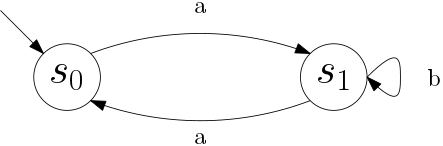
\includegraphics[scale=0.3]{Examples/ExamleVerification/LTSprojempty}
		\caption[LTS $M$]{LTS $M$}
		\label{fig:exverltsprojempty}
	\end{figure}

	The resulting parity game is depicted in figure \ref{fig:exverpg}. Let $V$ denote the set of vertices of this parity game. There are two vertices with more than one outgoing edge. From vertex $(s_1, [a](\mu X.\phi) \vee \langle b \rangle \top)$ player 0 does not want to play to $(s_1, \langle b \rangle \top)$ because he/she will not be able to make another move and looses the path. From vertex $(s_2, [a](\mu X.\phi)  \vee \langle b \rangle \top)$ player 0 can play to $(s_2, \langle b \rangle \top)$ to bring the play in $(s_2,\top)$ to win the path. We get the following winning sets:
	\begin{align*}
	W_1 &= \{ (s_1, \langle b \rangle \top )\}\\
	W_0 &= V \backslash W_1
	\end{align*}
	With the strategies $\sigma_0$ for player $0$ and $\sigma_1$ for player $1$ being (vertices with one outgoing edge are omitted):
	\begin{align*}
	\sigma_0 = \{
	&(s_1, [a](\mu X. \phi) \vee \langle b \rangle \top) \mapsto (s_1, [a] (\mu X. \phi)), \\
	&(s_2, [a](\mu X. \phi) \vee \langle b \rangle \top) \mapsto (s_2, \langle b \rangle \top) \} \\
	\sigma_1 = \{&\}
	\end{align*}
	Note that the choice where to go from $(s_2, [a](\mu X.\phi) \vee \langle b \rangle \top)$ does not matter for the winning sets.
	\begin{figure}[h]
		\centering
		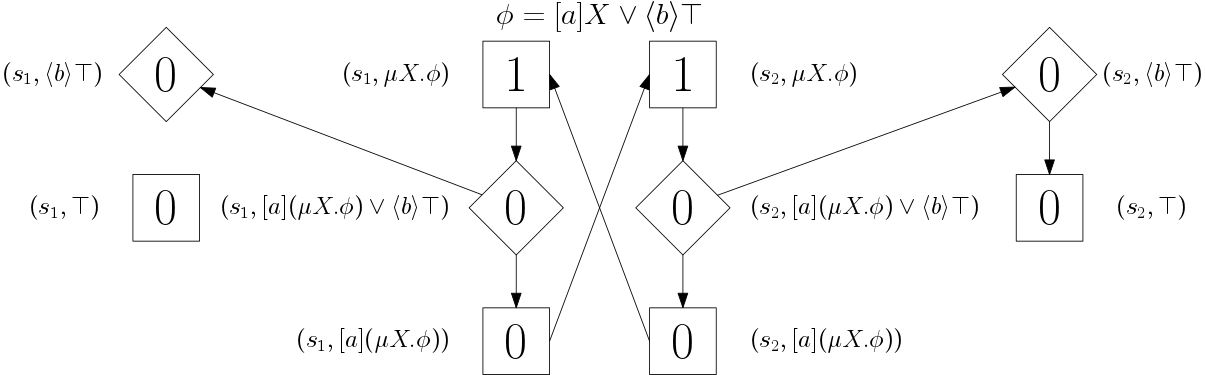
\includegraphics[scale=0.3]{Examples/ExamleVerification/PG}
		\caption[Parity game $LTS2PG(M, \varphi)$]{Parity game $LTS2PG(M, \varphi)$}
		\label{fig:exverpg}
	\end{figure}
\end{example}

Parity games created in this manner relate back to the model verification question; state $s$ in LTS $M$ satisfies $\varphi$ if and only if player $0$ wins vertex $(s, \varphi)$. This is formally stated in the following theorem which is proven in \cite{Bradfield2018}.
\begin{theorem}[\cite{Bradfield2018}]
	\label{the_LTS_PG_REL}Given LTS $M = (S, Act, trans, s_0)$, modal $\mu$-calculus formula $\varphi$ and state $s \in S$ it holds that $(M, s) \models \varphi$ if and only if $(s,\varphi) \in W_0$ for the game $LTS2PG(M, \varphi)$.
\end{theorem}

\subsection{Globally and locally solving parity games}
Parity games can be solved \textit{globally} or \textit{locally}; globally solving a parity game means that for every vertex in the game it is determined who the winner is. Locally solving a parity game means that for a specific vertex in the game it is determined who the winner is. For some applications of parity games, including model checking, there is a specific vertex that needs to be solved to solve the original problem. Locally solving the parity game is sufficient in such cases to solve the original problem.

Most parity game algorithms (including the two considered next) are concerned with globally solving, when talking about solving a parity game we talk about globally solving it unless stated otherwise. 

\subsection{Parity game algorithms}
Various algorithms for solving parity games are known, we introduce two of them. First Zielonka's recursive algorithm which is well studied and generally considered to be one of the best performing parity game algorithms in practice \cite{Oink,SolvingPGInPractice}. We also inspect the fixed-point iteration algorithm which tends to perform well for model-checking problems with a low number of distinct priorities \cite{BDDSolvingPG}.

\subsubsection{Zielonka's recursive algorithm}
First we consider Zielonka's recursive algorithm \cite{ZIELONKA1998135,MCNAUGHTON1993149}, which solves total parity games. Pseudo code is presented in algorithm \ref{alg_zlnk_org}. Zielonka's recursive algorithm has a worst-case time complexity of $O(e*n^d)$ where $e$ is the number of edges, $n$ the number of vertices and $d$ the number of distinct priorities.
\begin{algorithm}
	\caption{$\textsc{RecursivePG}(\textit{PG } G = (V,V_0,V_1, E, \Omega))$}
	\label{alg_zlnk_org}
	\begin{algorithmic}[1]
		\State $m \gets \min\{ \Omega(v)\ |\ v \in V\}$
		\State $h \gets\max\{ \Omega(v)\ |\ v \in V\}$
		\If{$h = m$ or $V = \emptyset$}
		\If{$h$ is even or $V = \emptyset$}
		\State \Return $(V,\emptyset)$
		\Else
		\State \Return $(\emptyset, V)$
		\EndIf
		\EndIf
		\State $\alpha \gets 0$ if $h$ is even and $1$ otherwise
		\State $U \gets \{v \in V\ |\ \Omega(v) = h\}$
		\State $A \gets \alpha\textit{-Attr}(G, U)$
		\State $(W_0', W_1') \gets \textsc{RecursivePG}(G \backslash A)$
		\If{$W_{\overline{\alpha}}' =\emptyset$}
		\State $W_\alpha \gets A \cup W_\alpha'$
		\State $W_{\overline{\alpha}} \gets \emptyset$
		\Else
		\State $B \gets \overline{\alpha}\textit{-Attr}(G,W_{\overline{\alpha}}')$
		\State $(W_0'', W_1'') \gets \textsc{RecursivePG}(G \backslash B)$
		\State $W_\alpha \gets W_\alpha''$
		\State $W_{\overline{\alpha}} \gets W_{\overline{\alpha}}'' \cup B$
		\EndIf
		\State \Return $(W_0, W_1)$
	\end{algorithmic}
\end{algorithm}

The algorithm solves $G$ by taking the set of vertices with the highest priority and choosing player $\alpha$ such that $\alpha$ has the same parity as the highest priority. Next the algorithm finds set $A$ such that player $\alpha$ can force the play to one of these high priority vertices. Next this set of vertices is removed from $G$ and the resulting subgame $G'$ is solved recursively. 

If $G'$ is entirely won by player $\alpha$ then we distinguish three cases for any path played in $G$. Either the path eventually stays in $G'$, $A$ is infinitely often visited or the path eventually stays in $A$. In the first case player $\alpha$ wins because game $G'$ was entirely won by player $\alpha$. In the second and third case player $\alpha$ can play to the highest priority from $A$. The highest priority, which has parity $\alpha$, is visited infinitely often and player $\alpha$ wins.

If $G'$ is not entirely won by player $\alpha$ we consider winning sets $W'_0$ and $W'_1$ of subgame $G'$. Vertices in set $W'_{\overline{\alpha}}$ are won by player $\overline{\alpha}$ in $G'$ but are also won by player $\overline{\alpha}$ in $G$. The algorithm tries to find all the vertices in $G$ such that player $\overline{\alpha}$ can force the play to a vertex in $W'_{\overline{\alpha}}$ and therefore winning the game. We now have a set of vertices that are definitely won by player $\overline{\alpha}$ in game $G$. In the rest of the game player $\alpha$ can keep the play from $W'_{\overline{\alpha}}$ so the algorithm solves the rest of the game recursively to find the complete winning sets for game $G$.

A complete explanation of the algorithm can be found in \cite{ZIELONKA1998135}, we do introduce definitions for the attractor set and for subgames. 

An attractor set is a set of vertices $A \subseteq V$ calculated for player $\alpha$ given set $U \subseteq V$ where player $\alpha$ has a strategy to force the play starting in any vertex in $A \backslash U$ to a vertex in $U$. Such a set is calculated by adding vertices owned by player $\alpha$ that have an edge to the attractor set and adding vertices owned by player $\overline{\alpha}$ that only have edges to the attractor set.

\begin{definition}[\cite{ZIELONKA1998135}]
	\label{def_attr}Given parity game $G = (V,V_0,V_1,E,\Omega)$ and a non-empty set $U \subseteq V$ we define $\alpha\textit{-Attr}(G,U)$ such that
	\[U_0 = U \]
	For $i \geq 0$:
	\begin{align*}
	U_{i+1} = U_i\cup
	&\{v \in V_\alpha\ |\ \exists v' \in V : v' \in U_i \wedge (v,v') \in E \}\\
	\cup &\{v \in V_{\overline{\alpha}}\ |\ \forall v' \in V :(v,v') \in E \implies v' \in U_i \}
	\end{align*}
	Finally:
	\[\alpha\textit{-Attr}(G,U) = \bigcup_{i \geq 0} U_i \]
\end{definition}

\begin{figure}
	\centering
	\begin{subfigure}{1\textwidth}
		\centering
		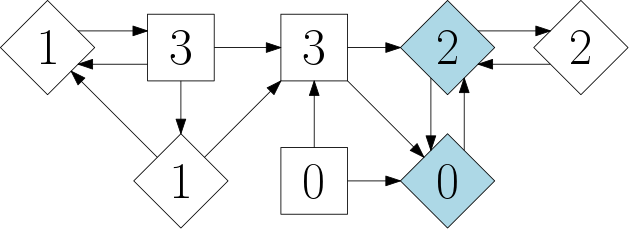
\includegraphics[scale=0.4]{Examples/Attr/Attr0}
		\caption{Set $U = U_0$}
	\end{subfigure}\\
	\begin{subfigure}{1\textwidth}
		\centering
		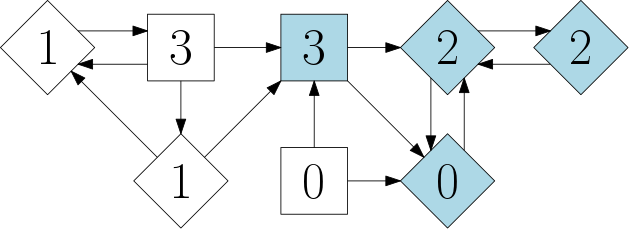
\includegraphics[scale=0.4]{Examples/Attr/Attr1}
		\caption{Set $U_1$}
	\end{subfigure}\\
	\begin{subfigure}{1\textwidth}
		\centering
		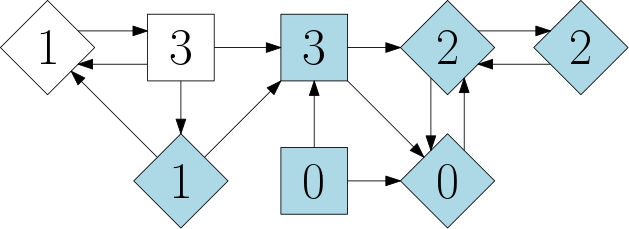
\includegraphics[scale=0.4]{Examples/Attr/Attr2}
		\caption{Set $U_2 = 0\textit{-Attr}(G,U)$}
	\end{subfigure}
	\caption{Game $G$ showing the attractor calculation for $0\textit{-Attr}(G,U)$}
	\label{fig:AttrCalcExample}
\end{figure}
\begin{example}
	Figure \ref{fig:AttrCalcExample} shows an example parity game in which an attractor set is calculated for player $0$. For set $U_2$ no more vertices can be attracted so we found the complete attractor set.
\end{example}

The algorithm also creates subgames, where a set of vertices is removed from a parity game to create a new parity game.

\begin{definition}[\cite{ZIELONKA1998135}]
	\label{def_org_subgame}
	Given a parity game $G = (V,V_0,V_1, E,\Omega)$ and $U \subseteq V$ we define the subgame $G \backslash U$ to be the game $(V', V_0', V_1', E', \Omega)$ with:
	\begin{itemize}
		\item $V' = V \backslash U$,
		\item $V_0' = V_0 \cap V'$,
		\item $V_1' = V_1 \cap V'$ and
		\item $E' = E \cap (V' \times V')$.
	\end{itemize}
\end{definition}

Note that a subgame is not necessarily total, however the recursive algorithm always creates subgames that are total (shown in \cite{ZIELONKA1998135}).

\subsubsection{Fixed-point iteration algorithm}
Parity games can be solved by solving an alternating fixed-point formula \cite{WALUKIEWICZ2002311}. Consider PG $G = (V,V_0,V_1, E, \Omega)$ with $d$ distinct priorities. We can apply \textit{priority compression} to make sure every priority in $G$ maps to a value in $\{0,\dots,d-1\}$ or $\{1, \dots, d\}$ \cite{SolvingInPractice,FPITE}. We assume without loss of generality that the priorities map to $\{0,\dots,d-1\}$ and that $d-1$ is even. 

Consider the following formula
\[ S(G = (V,V_0,V_1,E,\Omega)) = \nu Z_{d-1}. \mu Z_{d-2}. \dots . \nu Z_0. F_0(Z_{d-1},\dots,Z_0) \]
with
\[ F_0(Z_{d-1},\dots,Z_0) = \{ v \in V_0\ |\ \exists_{w\in V} (v,w) \in E \wedge Z_{\Omega(w)} \} \cup \{ v \in V_1\ |\ \forall_{w\in V} (v,w) \in E \implies Z_{\Omega(w)} \} \]
where $Z_i \subseteq V$. The formula $\nu X. f(X)$ solves the greatest fixed-point of $X$ in $f$, similarly $\mu X.f(X)$ solves the least fixed-point of $X$ in $f$. As shown in \cite{WALUKIEWICZ2002311} formula $S(G)$ is calculates the set of vertices winning for player 0 in parity game $G$.

To understand the formula we consider sub-formula $\nu Z_0. F_0(Z_{d-1},\dots,Z_0)$. This formula holds for vertices from which player $0$ can either force the play into a node with priority $i > 0$ for which $Z_i$ holds or the player can stay in vertices with priority $0$ indefinitely. The formula $\mu Z_0. F_0(Z_{d-1},\dots,Z_0)$ holds for vertices from which player $0$ can force the play into a node with priority $i > 0$, for which $Z_i$ holds in finitely many steps. By alternating fixed-points the formula allows infinitely many consecutive stays in even vertices and finitely many consecutive stays in odd vertices. For an extensive treatment we refer to \cite{WALUKIEWICZ2002311}.

We further inspect formula $S$. Given game $G$, consider the following sub-formulas:
\[ S^{d-1}(Z_{d-1}) = \mu Z_{d-2}.S^{d-2}(Z_{d-2})\]
\[ S^{d-2}(Z_{d-2}) = \nu Z_{d-3}.S^{d-3}(Z_{d-3})\]
\begin{center}
	\dots
\end{center}
\[ S^{0}(Z_0) = F_0(Z_{d-1},\dots,Z_0)\]
The fixed-point variables are all elements of $2^V$, therefore we have for every sub-formula the following type:
\[ S^i(Z_i) : 2^V \rightarrow 2^V \]
Furthermore, since $V$ is finite, the partially ordered set $\langle 2^V, \subseteq \rangle$ is a complete lattice; for every subset $X \subseteq 2^V$ we have infimum $\bigcap_{x \in X} x$ and supremum $\bigcup_{x \in X} x$. Finally every sub-formula $S^i(Z_i)$ is monotonic, ie. if $S^i(Z_i) \geq S^i(Z_i')$ then $Z_i \geq Z_i'$.

Fixed-point formula's can be solved by \textit{fixed-point iteration}. As shown in \cite{Emerson:1986:MCP:900378} we can calculate $\mu X.f(X)$, where $f$ is monotonic in $X$ and $X \in 2^V$, by iterating $X$:
\[ \mu X.f(X) = \bigcup_{i \geq 0} X^i \]
where $X^i = f(X^{i-1})$ for $i > 0$ and $X^0 \subseteq \mu X.f(X)$. So picking the smallest value possible for $X_0$ will always correctly calculate $\mu X. f(X)$.

Similarly we can calculate fixed-point $\nu X.f(X)$ when $f$ is monotonic in $X$ by iterating $X$:
\[ \nu X.f(X) = \bigcap_{i \geq 0} X^i \]
where $X^i = f(X^{i-1})$ for $i > 0$ and $X^0 \supseteq \nu X.f(X)$. So picking the largest value possible for $X_0$ will always correctly calculate $\nu X. f(X)$.

Since every subformula is monotonic and maps from a value in $2^V$ to another value in $2^V$ we can apply fixed-point iteration to solve the subformula's, we choose initial values $\emptyset$ for least fixed-point variables and $V$ for greatest fixed-point variables.

An algorithm to perform the iteration is presented in \cite{FPITE} and shown in algorithm \ref{alg_FPITEorg}. This algorithm has a worst-case time complexity of $O(e * n ^d)$ where $e$ is the number of edges, $n$ the number of vertices and $d$ the number of distinct priorities.
\begin{algorithm}
	\caption{Fixed-point iteration}
	\label{alg_FPITEorg}
	\begin{multicols}{2}
		\begin{algorithmic}[1]
			\Function{FPIter}{$G = (V, V_0, V_1, E, \Omega)$}
			\For{$i \gets d-1,\dots,0$}
			\State $\textsc{Init}(i)$
			\EndFor
			\Repeat
			\State $Z_0'\gets Z_0$
			\State $Z_0 \gets \textsc{Diamond}() \cup \textsc{Box}()$
			\State $i \gets 0$
			\While{$Z_i=Z_i' \wedge i < d-1$}
			\State $i \gets i+1$
			\State $Z_i' \gets Z_i$
			\State $Z_i \gets Z_{i-1}$
			\State $\textsc{Init}(i-1)$
			\EndWhile
			\Until{$i = d-1 \wedge Z_{d-1} = Z_{d-1}'$}
			\State \Return $(Z_{d-1},V\backslash Z_{d-1})$
			\EndFunction
		\end{algorithmic}\bigskip\bigskip
		\begin{algorithmic}[1]
			\Function{Init}{$i$}
			\State $Z_i \gets \emptyset$ if $i$ is odd, $V$ otherwise
			\EndFunction
		\end{algorithmic}\bigskip
		\begin{algorithmic}[1]
			\Function{Diamond}{}
			\State \Return $\{ v \in V_0\ |\ \exists_{w\in V} (v,w) \in E \wedge w \in Z_{\Omega(w)}\}$
			\EndFunction
		\end{algorithmic}\bigskip
		\begin{algorithmic}[1]
			\Function{Box}{}
			\State \Return $\{ v \in V_1\ |\ \forall_{w\in V} (v,w) \in E \implies w \in Z_{\Omega(w)}\}$
			\EndFunction
		\end{algorithmic}
	\end{multicols}
\end{algorithm}

\section{Symbolically representing sets}
A set can straightforwardly be represented by a collection containing all the elements that are in the set. We call this an \textit{explicit} representation of a set. We can also represent sets \textit{symbolically} in which case the set of elements is represented by some sort of formula. A typical way to represent a set symbolically is through a boolean formula encoded in a \textit{binary decision diagram} \cite{BDD_book,Handbook_BDD_Chapter}. 

\begin{example}
	\label{ex_boolform}
	The set $S = \{ 2,4,6,7 \}$ can be expressed by boolean formula:
	\[ F(x_2,x_1,x_0) = (\neg x_2 \wedge x_1 \wedge \neg x_0) \vee (x_2 \wedge (x_1 \vee \neg x_0)) \]
	where $x_0,x_1$ and $x_2$ are boolean variables. The formula gives the following truth table:\\
	\begin{center}
		\begin{tabular}{|c|c|}
			\hline 
			$\mathbf{x_2x_1x_0}$ & $\mathbf{F(x_2,x_1,x_0)}$ \\ 
			\hline 
			000 & 0 \\ 
			\hline 
			001 & 0 \\ 
			\hline 
			010 & 1 \\ 
			\hline 
			011 & 0 \\ 
			\hline 
			100 & 1 \\ 
			\hline 
			101 & 0 \\ 
			\hline 
			110 & 1 \\ 
			\hline 
			111 & 1 \\ 
			\hline
		\end{tabular} 
	\end{center}
	The function $F$ defines set $S'$ in the following way: $S' = \{x_2x_1x_0\ |\ F(x_2,x_1,x_0) = 1 \}$. As we can see set $S'$ contains the same numbers as $S$ but represented binary.
\end{example}
We can perform set operations on sets represented as boolean functions by performing logical operations on the functions. For example, given boolean formula's $f$ and $g$ representing sets $V$ and $W$ the formula $f \wedge g$ represents set $V \cap W$.

Given a set $S$ with arbitrary elements we can represent subsets $S' \subseteq S$ as boolean formula's by assigning a number to every element in $S$ and creating a boolean formula that maps boolean variables to true if and only if they represent a number such that the element associated with this number in $S$ is also in $S'$.

\subsection{Binary decision diagrams}
A boolean function can efficiently be represented as a binary decision diagram (BDD), for a comprehensive treatment of BDDs we refer to \cite{BDD_book,Handbook_BDD_Chapter}.

BDDs represent boolean formula's as a directed graph where every vertex represents a boolean variable and has two outgoing edges labelled 0 and 1. Furthermore the graph contains special vertices $0$ and $1$ that have no outgoing edges. We decide if a boolean variable assignment satisfies the formula by starting in the initial vertex of the graph and following a path until we get to either vertex 0 or 1. Since every vertex represents a boolean formula we can create a path from the initial vertex by choosing edge 0 at a vertex if the boolean variable represented by that vertex is false in the variable assignment and choosing edge 1 if is true. Eventually we end up in either vertex 0 or 1. In the former case the boolean variable assignment does not satisfy the formula, in the latter it does.

\begin{example}
	Consider the boolean formula in example \ref{ex_boolform}. This formula can be represented as the BDD shown in Figure \ref{fig:ex_simplebdd}. The vertices representing boolean variables are shown as circles and the boolean variables they represent are indicated inside them. The special vertices are represented as squares and the initial vertex is represented by an edge with that has no origin vertex.
\begin{figure}[h]
	\centering
	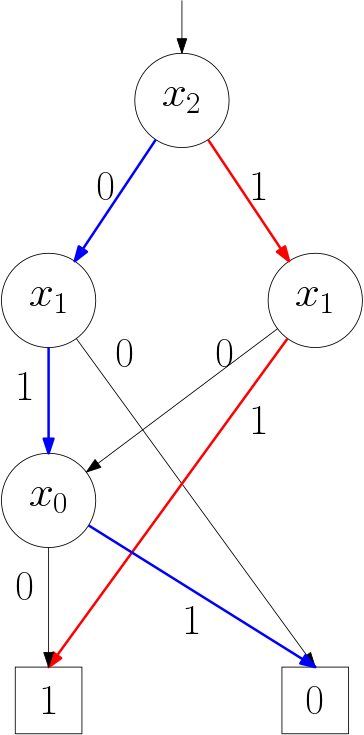
\includegraphics[scale=0.3]{Examples/BDD/simpleexample}
	\caption{BDD highlighting boolean variable assignment $x_2x_1x_0 = 011$ in blue and $x_2x_1 = 11$ in red}
	\label{fig:ex_simplebdd}
\end{figure}
	
	The path created from variable assignment $x_2x_1x_0 = 011$ is highlighted in blue in the diagram and shows that this assignment is indeed not satisfied by the boolean formula. The red path shows the variable assignments $110$ and $111$. Determining the path and the outcome for every variable assignment results in the same truth table as seen in example \ref{ex_boolform}.
\end{example}

Given $n$ boolean variables and two boolean functions encoded as BDDs we can perform binary operations $\vee,\wedge$ on the BDDs in $O(2^{2n})=O(m^2)$ where $m = 2^n$ is the maximum set size that can be represented by $n$ variables \cite{BDD_running_time,Handbook_BDD_Chapter}. The running time specifically depends on the size of the decision diagrams, in general if the boolean functions are simple then the size of the decision diagram is also small and operations can be performed quickly.